\documentclass[ignorenonframetext,red,8pt]{beamer}

\usepackage[utf8]{inputenc}
\usepackage{beamerthemesplit}
\usepackage{graphics}
\usepackage{natbib}
\usepackage[english]{babel}
\usepackage{url}
\usepackage{times}
\usepackage[T1]{fontenc}
\usepackage{hyperref}
\usepackage{epstopdf}
\usepackage{subfig}

\usepackage{multirow}
\usepackage{rotating}

% hack for beamer and natbib working together
%\newcommand{\newblock}{}

\mode<presentation>
{
	\usetheme{Warsaw}
% 	\usecolortheme{lily}
}

\mode<article>
{
  \usepackage{fullpage}
  \usepackage{pgf}
%  \setjobnamebeamerversion{beamerexample2.beamer}
}

\usepackage{fancyvrb}
\usepackage{color}
%\usepackage{colortbl}
\usepackage{listings}
%\usepackage{listings,bera}
\definecolor{keywords}{RGB}{128,148,182}
%\definecolor{comments}{RGB}{60,179,113}
\definecolor{comments}{RGB}{0,0,139}
\lstset{language=Python,
        %numbers=false,
        showstringspaces=false,
        numberstyle=\tiny,
        %frame=leftline,
        numbersep=4.5pt,
  keywordstyle=\color{keywords}\bfseries,
  commentstyle=\color{comments}\emph
}

\hypersetup{
%   pdfpagemode=FullScreen, % Sembla que no funciona correctament
  unicode=true,
  pdftitle={The Structural Dimension of Cooperation},%
  pdfauthor={Jordi Torrents},%
  pdfcreator={},%
  pdfproducer=PDFLaTeX,%
  pdfsubject={},%
  pdfkeywords={}%
}

%\AtBeginSection[]{\frame{\frametitle{Contents}\tableofcontents[current]}}

\title{The Structural Dimension of Cooperation}
\subtitle{Cooperation Networks as Cohesive Small Worlds}
\author{Jordi Torrents}
\institute{University of Barcelona}

\begin{document}

\begin{frame}[label=portada]
\maketitle
\end{frame}

%\begin{frame}[label=toc]
%\frametitle{Contents}
%\tableofcontents
%\end{frame}

\section{Large Scale Cooperation}

\begin{frame}[label=]
\frametitle{Research Question}

The last half of twentieth century has witnessed a key shift in the production process of knowledge. 

\begin{block}{Well established empirical fact about Cooperation}
\citet*{uzzi:2007a} show that until 1950s the likelihood that an important ---ie wildly cited--- paper or invention was developed by a single author was bigger than it was developed by a team. But this trend has experimented a shift in the last four decades. The rising importance of collective research and cooperation is illustrated by the fact that top cited papers are mostly created by teams in 2000s.
\end{block}

\begin{block}{Research question}
How does large scale cooperation work in knowledge intensive and technically complex production processes developed in new organizational environments, such as Free and Open Source Software projects, where loosely coupled individuals that rarely meet face to face have to coordinate through internet in order to produce world class software products.
\end{block}

\end{frame}


\subsection{Theoretical Approaches to Cooperation}
\begin{frame}[label=]
\frametitle{Theoretical Approaches to Cooperation}

\begin{columns}[c]
\begin{column}{0.5\textwidth}

\begin{block}{Macro level approach}
Cooperation as a macro level phenomenon in which the center of analysis is the collective or group \citep{marx:1990, adler:2006, adler:2015}.

\begin{itemize}

\item Focus on large organizations and groups: Collaborative Communities

%\item Key elements to explain Cooperation:

\begin{itemize}

\item Shared values and goals
\item Generalized trust
\item Authority forms

\end{itemize}
\end{itemize}
\end{block}
\end{column}

\begin{column}{0.5\textwidth}

\begin{block}{Micro level approach}
Cooperation as a micro level phenomenon in which the center of analysis is the dyad \citep{axelrod1981, watts:1999, eguiluz:2005}.

\begin{itemize}

\item Reductionist approach: Cooperation as an atomic process.

%\item Key elements to explain Cooperation:

\begin{itemize}

\item Strategic dyadic interactions.
\item Agent-based models.
\item Payoffs of different strategies.

\end{itemize}
\end{itemize}

\end{block}

\end{column}
\end{columns}

\begin{block}{A meso level approach to Cooperation}
Focus on Cooperation networks: patterns of relations that direct producers establish in the production process.
\begin{itemize}

\item Structural approach, that is, a network approach.

%\item Key elements to explain Cooperation:

\begin{itemize}

\item Sub-groups that are more connected internally than with the rest of the network. 
\item Longitudinal analysis of the formation and dissolution of these groups.
\item Key mechanisms to explain and understand large scale cooperation.

\end{itemize}
\end{itemize}
\end{block}

\end{frame}


\begin{frame}
\frametitle{Collaborative Communities as a macro approach}
A new form of community, qualitatively different from the traditional \emph{Gemeinschaft} and the modern \emph{Gesellschaft} \citep{tonnies:1974} 

\begin{block}{Collaborative Communities \citep{adler:2006}}
Novel organizational form ---both inside and outside large capitalist corporations--- strongly grounded on large scale cooperation which defy the traditional dichotomy between \textbf{hierarchy} and \textbf{market} as coordinating mechanisms.

\begin{itemize}
\item Generalized trust
\item Conscius cooperation and High individual interdependence
\item Shared values and Value-rational basis for legitimate authority 
\end{itemize}
\end{block}

\begin{block}{Network (structural) model for Collaborative Communities}

\begin{description}
\item[Cohesive Small World] Based on the well known Small World and Structural Cohesion Models. Which structural conditions enable trust and value congruence?
\end{description}

\begin{itemize}
\item Small Worlds: Local clusters connected by shortest paths.
\item Structural Cohesion: Increasingly cohesive groups nested inside each other.
\end{itemize}
\end{block}

\end{frame}

\subsection{Cohesive Small Worlds}

\begin{frame}
\frametitle{Cohesive Small World}

\begin{columns}[c]
\begin{column}{0.33\textwidth}
\begin{center}
\textbf{Pure Structural Cohesion}
\end{center}
\begin{itemize}
\item Robust to node removal
\item Not necessary short average distance
\item Not necessary local clustering 
\end{itemize}
\includegraphics[scale=0.2]{../../figures/model_structural_cohesion_25}
\end{column}

\begin{column}{0.33\textwidth}
\begin{center}
\textbf{Cohesive Small World}
\end{center}
\begin{itemize}
\item Intersection of the two models
\item Short average distance
\item High local cluster coefficient
\item Robust to node removal
\end{itemize}
\includegraphics[scale=0.2]{../../figures/model_cohesive_small_world_25}
\end{column}

\begin{column}{0.33\textwidth}
\begin{center}
\textbf{Pure Small World}
\end{center}
\begin{itemize}
\item Short average distance
\item High local cluster coefficient
\item Not necessary robust to node removal
\end{itemize}
\includegraphics[scale=0.2]{../../figures/model_small_world_25}
\end{column}
\end{columns}

\end{frame}


\subsection{Structural cohesion model}

\begin{frame}
\frametitle{The structural cohesion model}

The structural cohesion model \citep{white:2001,moody:2003} is based on two mathematically equivalent definitions of cohesion.

\begin{block}{Precise definition of group cohesion based on \textbf{node connectivity}}

\begin{itemize}

\item a group's structural cohesion is equal to the minimum number of actors who, if removed from the group, would disconnect the group.

\item a group's structural cohesion is equal to the minimum number of node independent paths linking each pair of actors in the group.

\end{itemize}
\end{block}

This equivalence relation has a deep sociological meaning because it allows to define structural cohesion in terms of:

\begin{itemize}

\item the difficulty to pull a group apart by removing actors.

\item multiple relations between actors that keep a group together.

\end{itemize}
\end{frame}

\begin{frame}
\frametitle{Measures of structural cohesion}

%\begin{block}{Local node connectivity $\kappa_{G}(u,v)$}
%Given two nodes $u$ and $v$, $\kappa_{G}(u,v)$ is the minimum number of nodes that must be removed to destroy all paths that join $u$ and $v$.
%\end{block}

\begin{block}{Node connectivity $\kappa(G)$}
\begin{description}
\item[Local] given two nodes $u$ and $v$, $\kappa_{G}(u,v)$ is the minimum number of nodes that must be removed to destroy all paths that join $u$ and $v$.

\item[Global] the minimum number of nodes that must be removed in order to disconnect a graph $G$.

%\begin{equation*}
%\kappa = min{\{\kappa_{G}(u,v):u,v \in V(G)\}}
%\end{equation*}

\end{description}

\end{block}

%\begin{block}{Average node connectivity $\bar{\kappa}(G)$}
%the sum of local node connectivity between all pairs of different nodes of $G$ divided by the number of distinct pairs of nodes. \citep*{beineke:2002}.

%\begin{equation*}
%\bar{\kappa}(G) = \frac{\sum_{u,v} \kappa_{G}(u,v)}{{n \choose 2}}
%\end{equation*}
%\end{block}

\begin{block}{$k$-components}
A $k$-component is a maximal subgraph that has, at least, node connectivity $k$: we need to remove at least $k$ nodes to break it into more components. 
\end{block}

\begin{center}
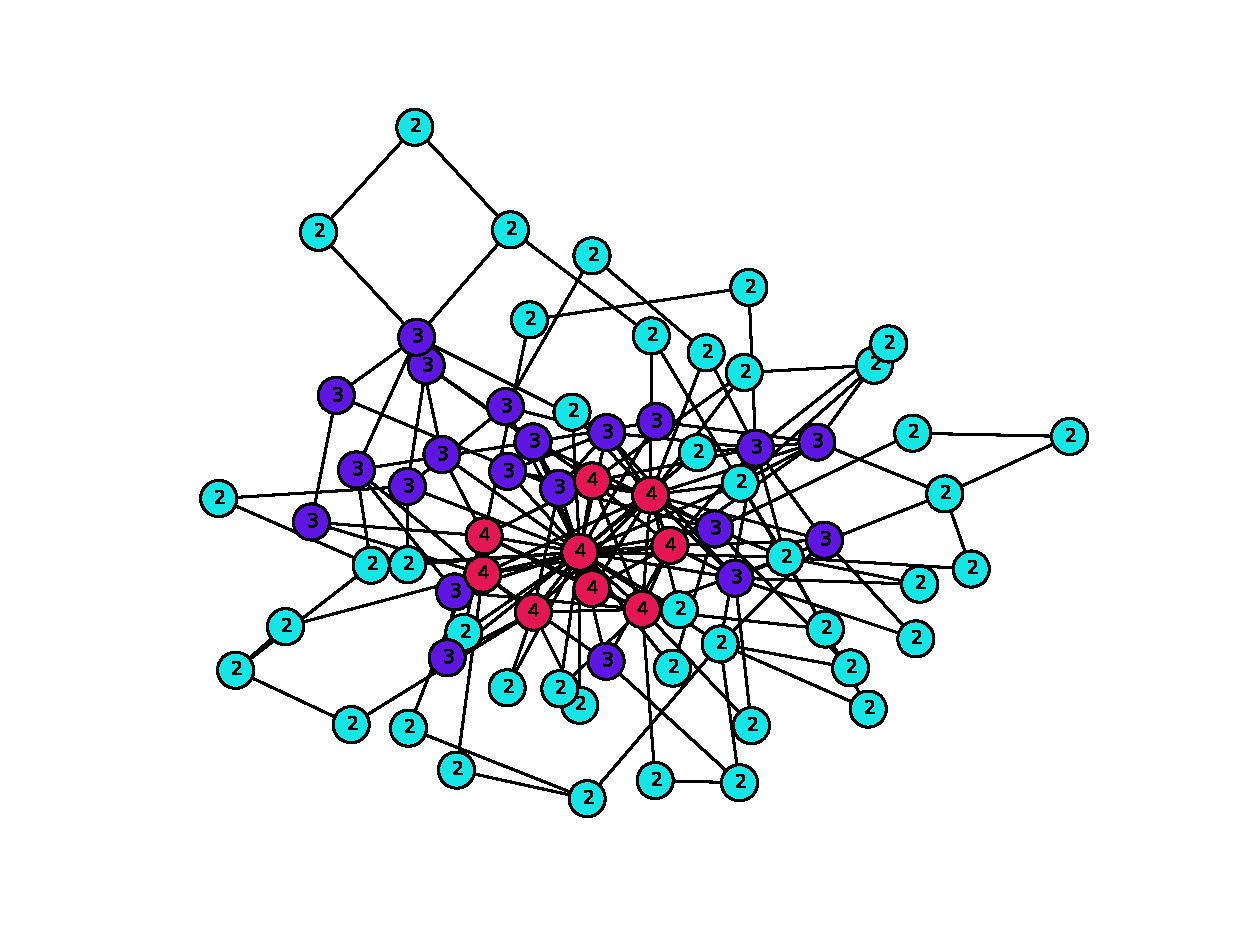
\includegraphics[scale=0.25]{img/knum_colors}
\end{center}

\end{frame}

\section{Empirical analysis: FOSS projects}

\subsection{Debian and Python}

\begin{frame}
\frametitle{Free and Open Source Projects: Debian and Python}

Free Software, broadly defined, is computer software that allows users to run, copy, distribute, study, change and improve it.

\begin{columns}[c]
\begin{column}{0.5\textwidth}
\begin{block}{The Debian Project: 1999-2012}
\begin{itemize}
\item A free Operating System
\item 392 developers in 1999, 1435 in 2012 
\item 2876 programs in 1999, 10469 in 2012
\item Widely used in servers (google), desktops (Ubuntu) and embedded devices (raspberry pi)
\end{itemize}
\end{block}
\end{column}

\begin{column}{0.5\textwidth}
\begin{block}{The Python project: 1999-2014}
\begin{itemize}
\item A free Programming Language
\item 9 developers in 1999, 62 in 2014
\item 1137 files in 1999, 2134 in 2014 
\item Widely used in web development (reddit, youtube) and scientific computing
\end{itemize}
\end{block}
\end{column}
\end{columns}

\begin{block}{Building and Analyzing Cooperation Networks}
\begin{itemize}
\item Cooperation networks are bipartite or two mode (both developers and programs)
\item A developer is linked to the package or source code file that she works on
\item Structural Cohesion Analysis: $\kappa$-components as sub-groups
\item Small World Analysis: Average Path Length and Clustering Coefficient 
\end{itemize}
\end{block}

\end{frame}

\subsection{Structural Cohesion Analysis}

\begin{frame}
\frametitle{Structural Cohesion Analysis}

\begin{columns}[c]
\begin{column}{0.5\textwidth}
\begin{center}
\textbf{Debian Cooperation Network 2004}
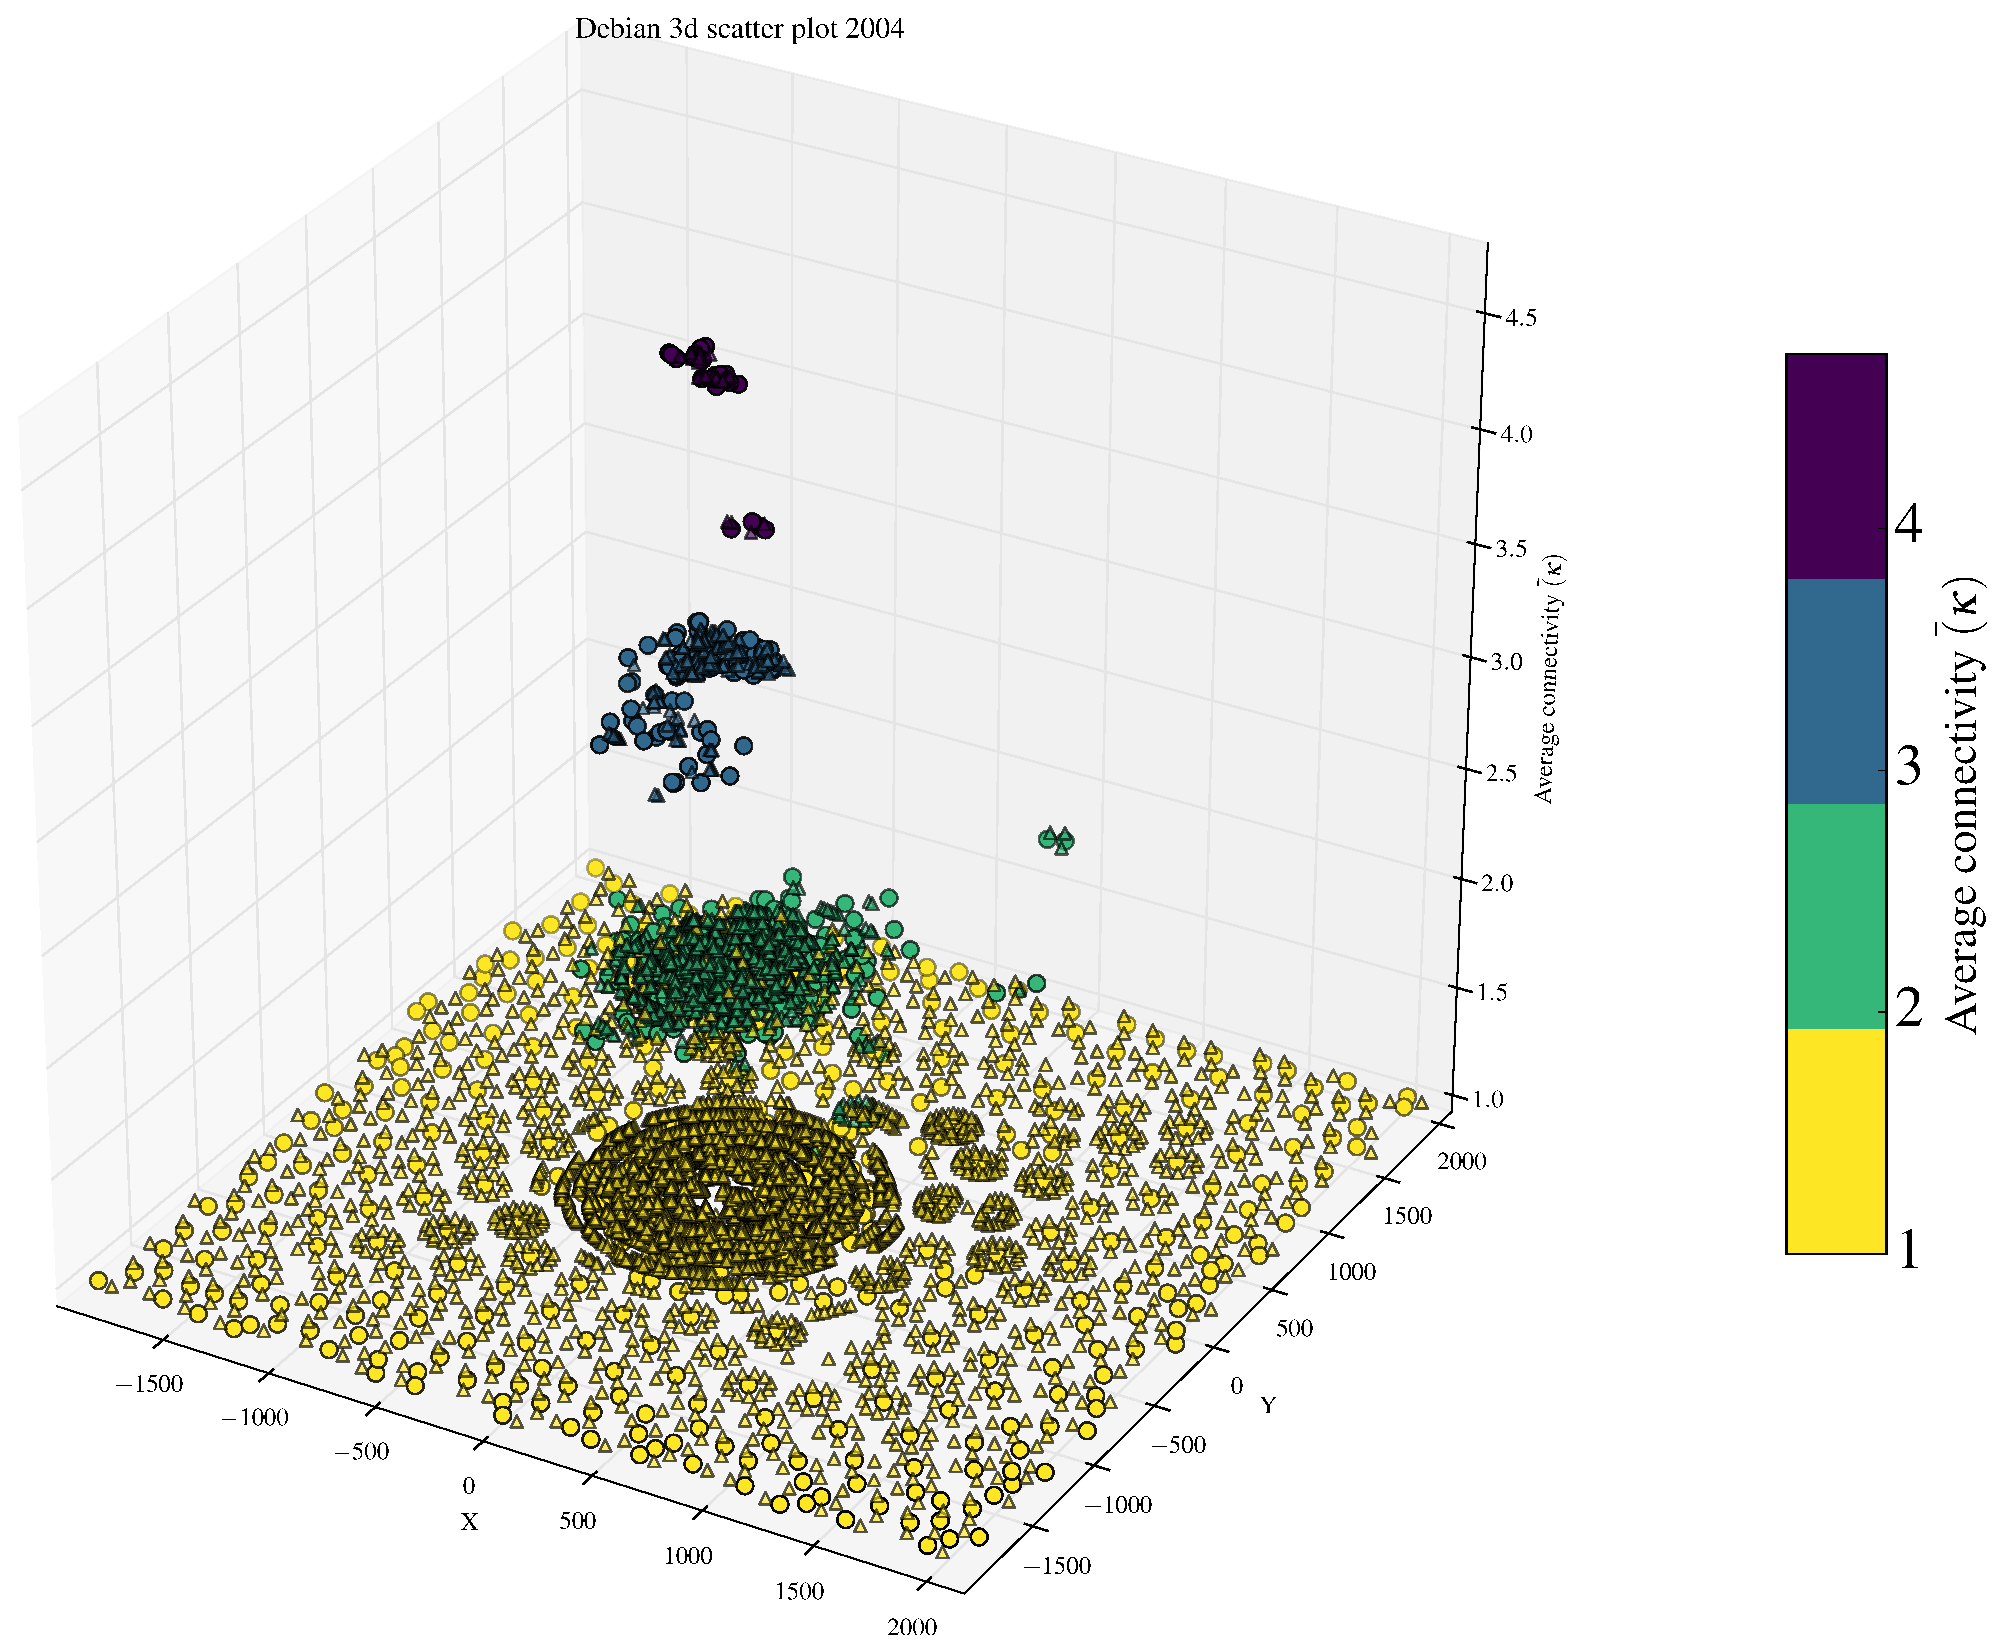
\includegraphics[scale=0.12]{../../figures/3d_scatter_debian_2004}
\newline
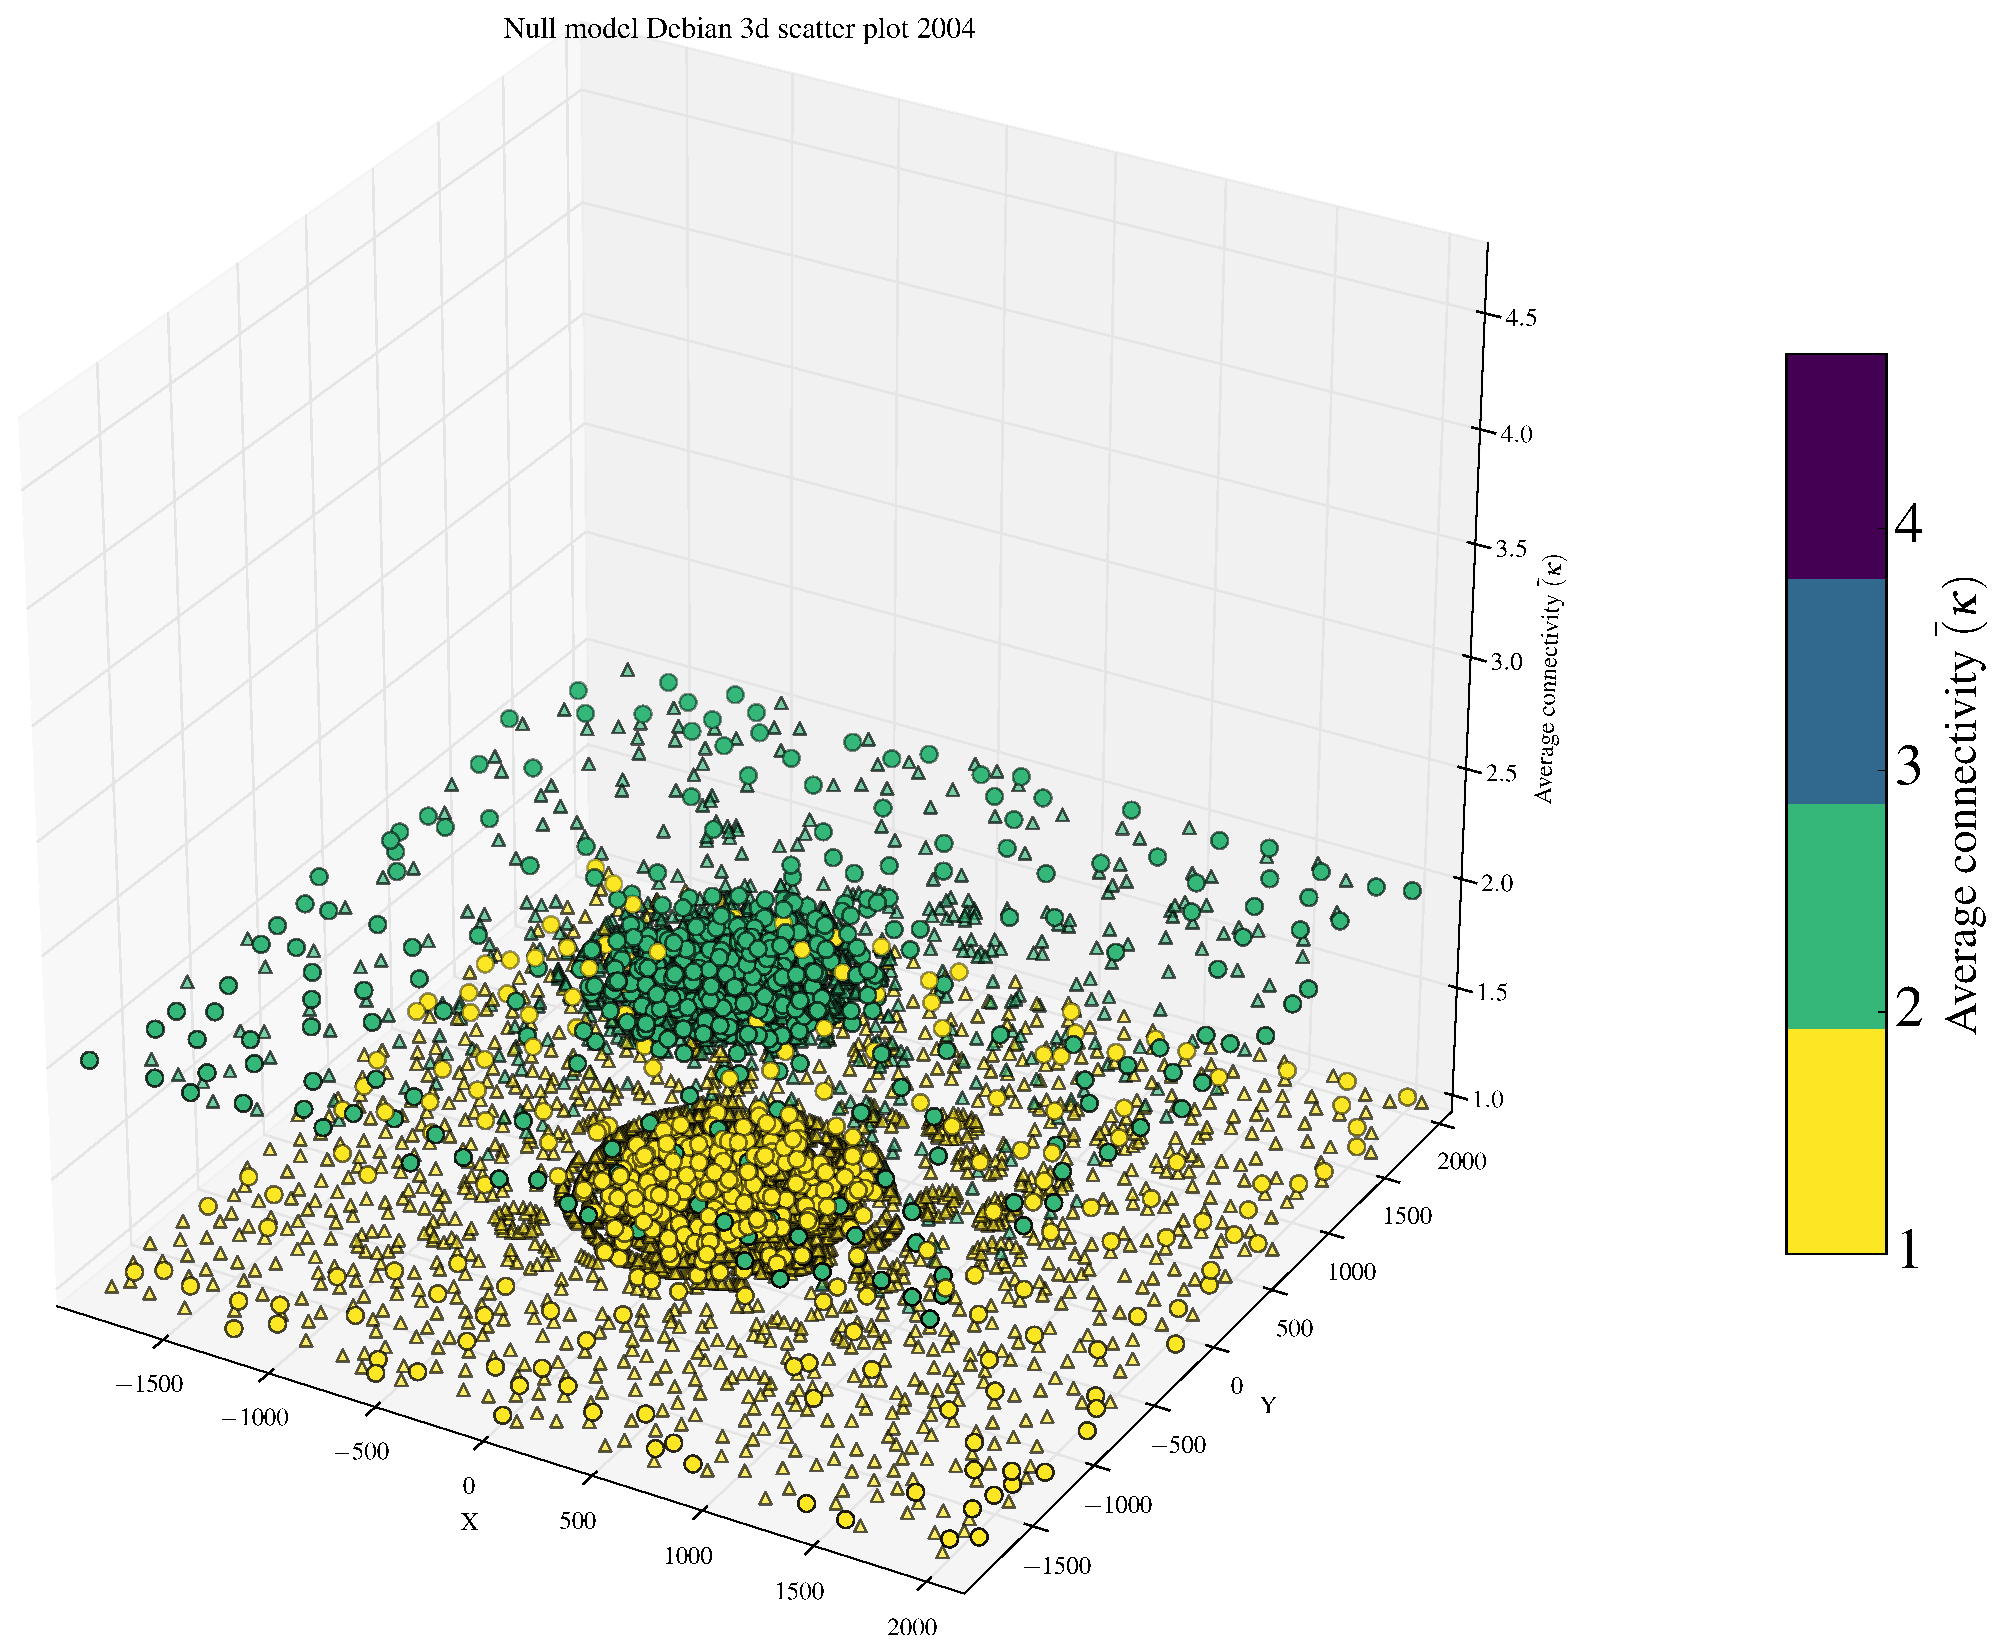
\includegraphics[scale=0.12]{../../figures/3d_scatter_debian_2004_null}
\end{center}
\end{column}

\begin{column}{0.5\textwidth}
\begin{center}
\textbf{Python Cooperation Network 2004}
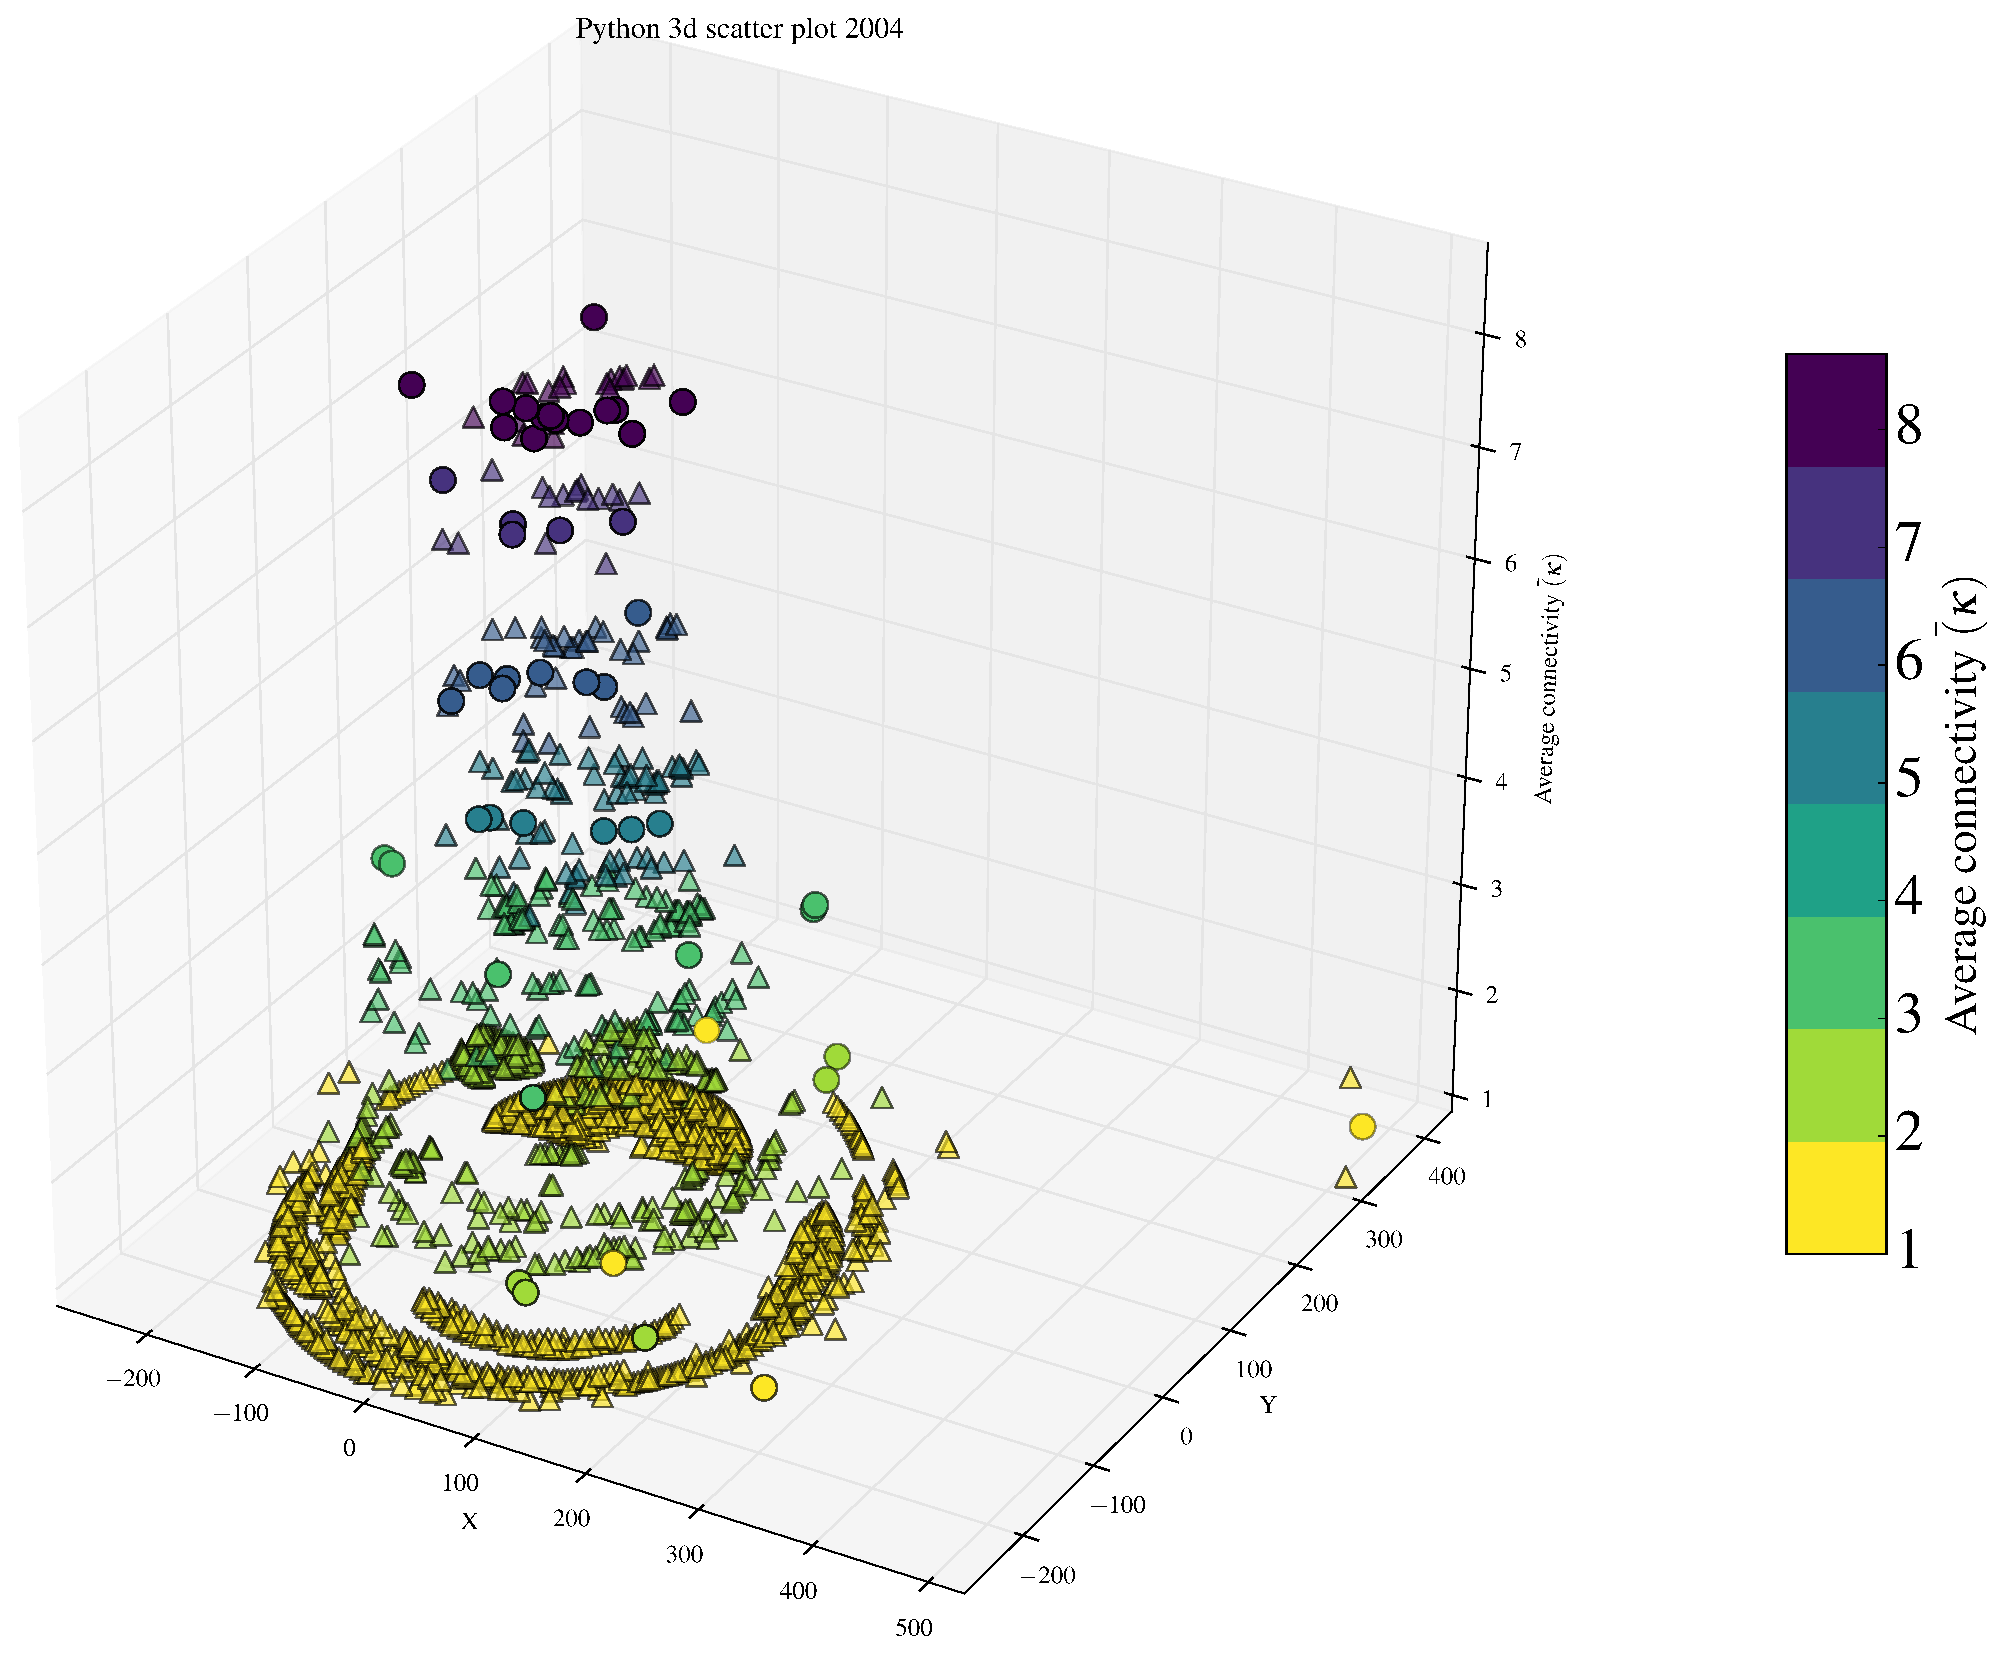
\includegraphics[scale=0.12]{../../figures/3d_scatter_python_2004}
\newline
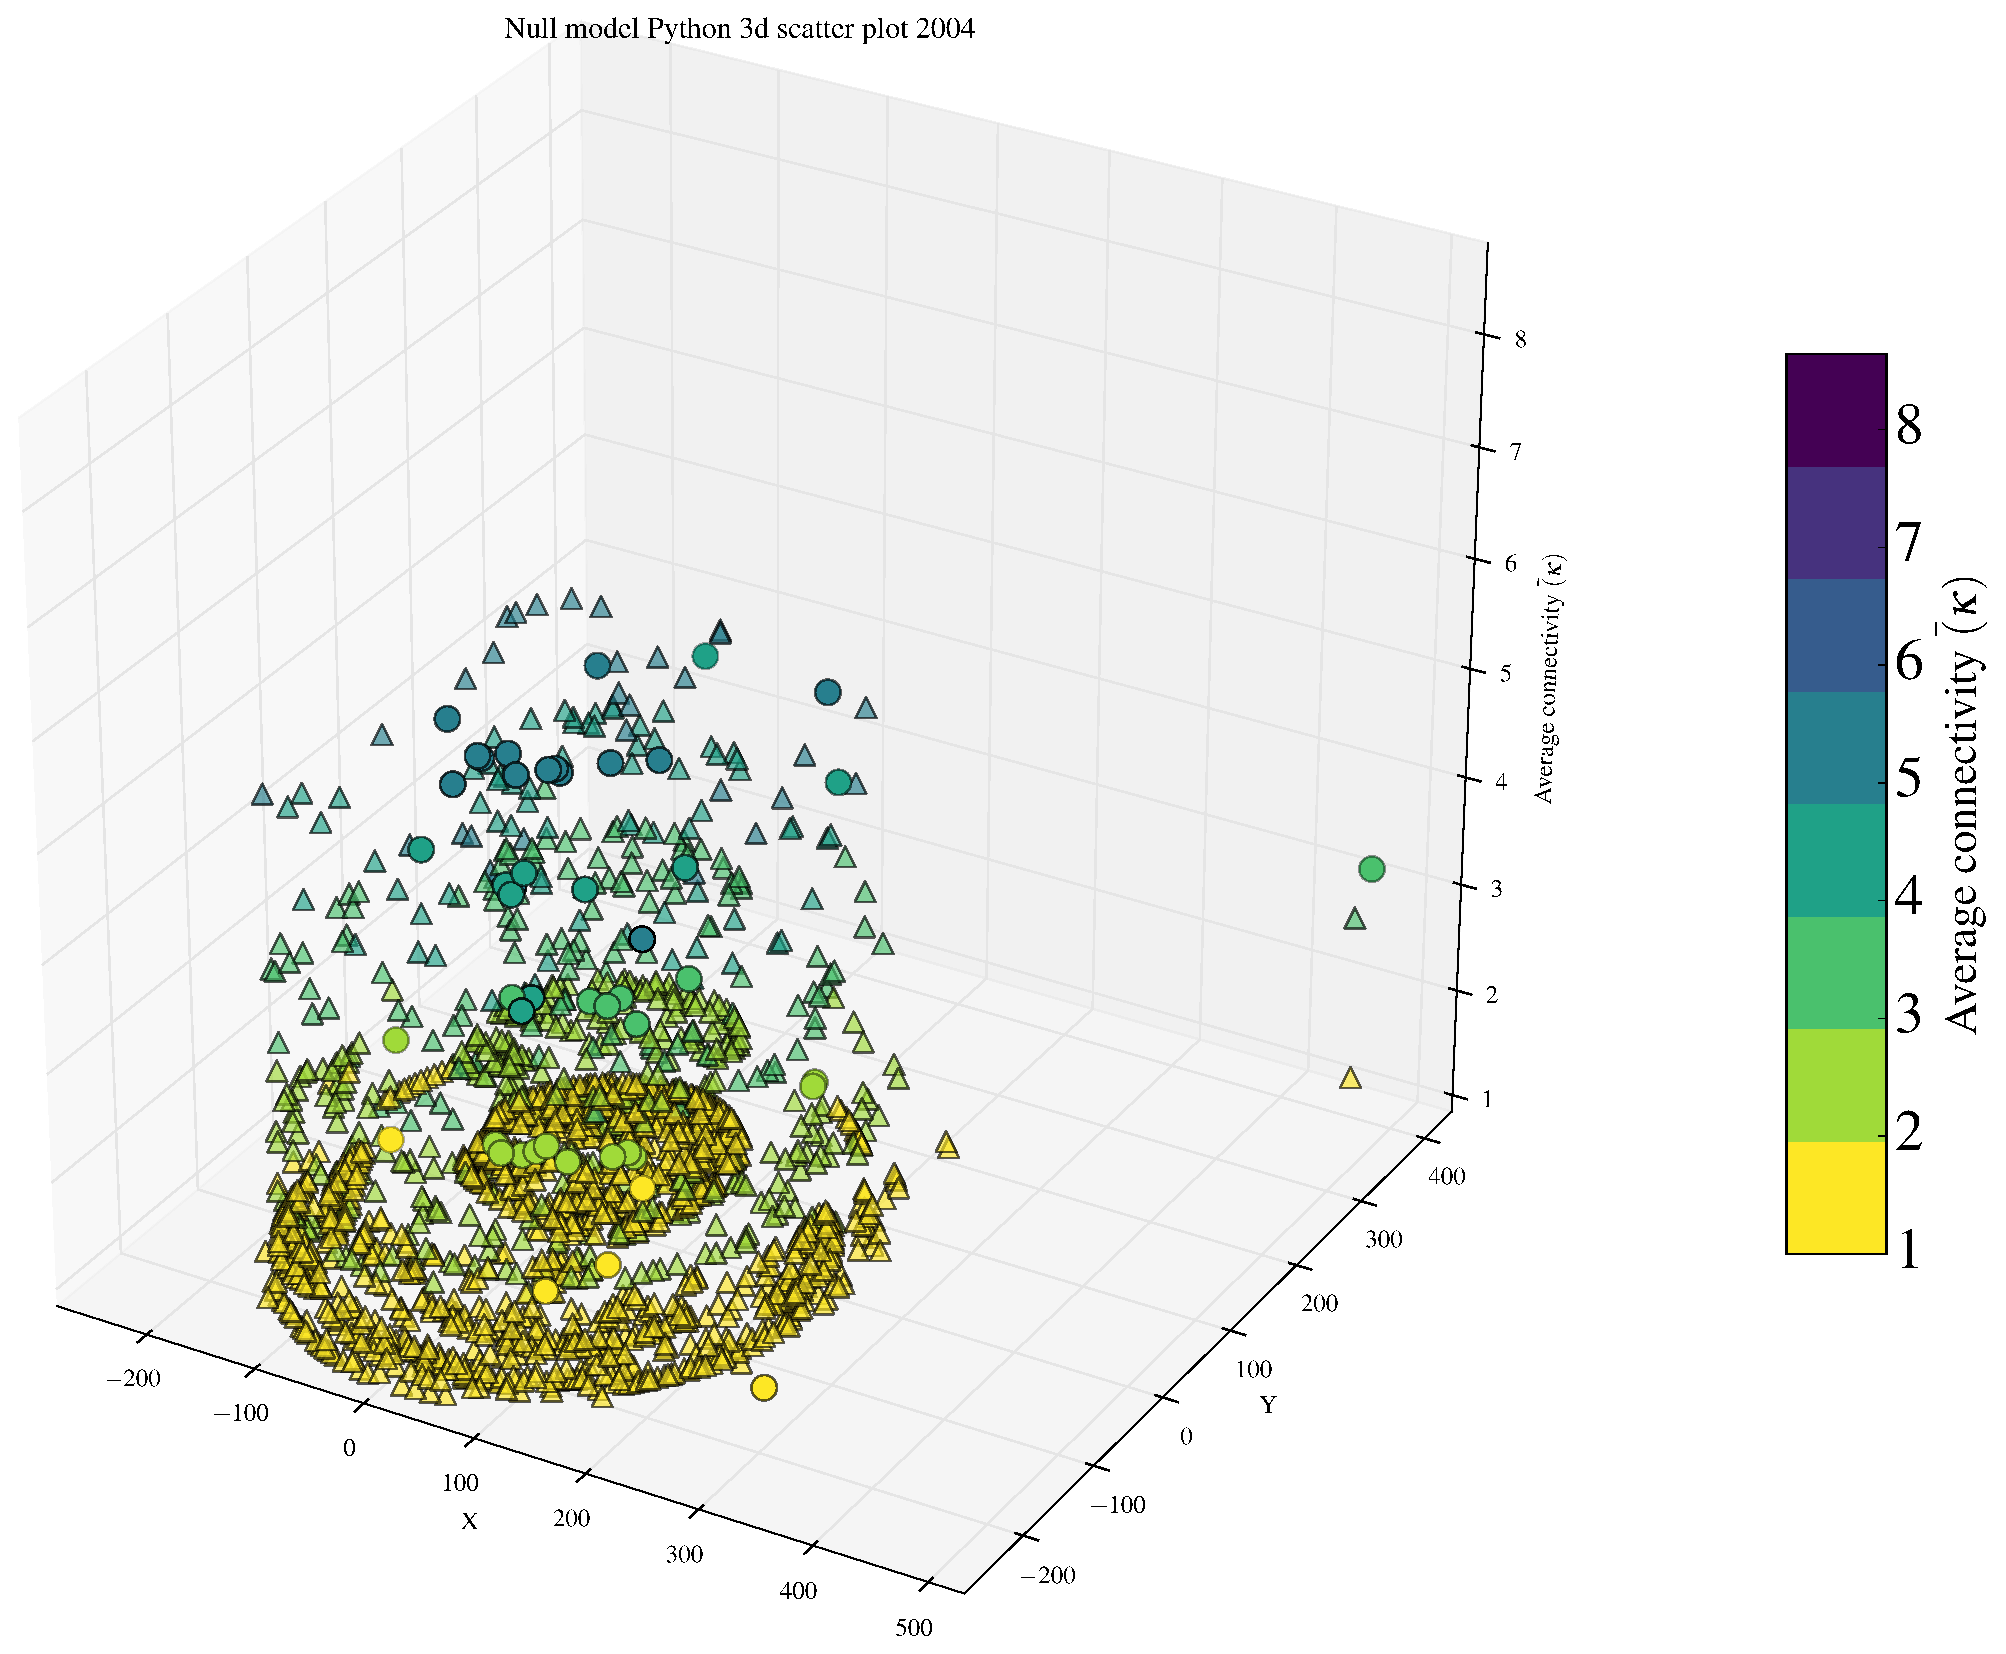
\includegraphics[scale=0.12]{../../figures/3d_scatter_python_2004_null}
\end{center}
\end{column}
\end{columns}

\end{frame}

\subsection{Analysis of Individual Contributions}

\begin{frame}
\frametitle{Iron law of the Oligarchy or an Open Elite?}

The literature on FOSS, especially from software engineering and computer science, have stressed that only a small fraction of the developers is doing most of the work.

\begin{columns}[c]
\begin{column}{0.5\textwidth}
\begin{center}
\textbf{Debian Contributions}
\includegraphics[scale=0.16]{../../figures/evolution_developers_debian_years}
\newline
\includegraphics[scale=0.16]{../../figures/evolution_connectivity_debian_years}
\end{center}
\end{column}

\begin{column}{0.5\textwidth}
\begin{center}
\textbf{Python Contributions}
\includegraphics[scale=0.16]{../../figures/evolution_developers_python_years}
\newline
\includegraphics[scale=0.16]{../../figures/evolution_connectivity_python_years}
\end{center}
\end{column}
\end{columns}
\end{frame}


\begin{frame}
\frametitle{Cooperation Networks' Connectiviy Hierarchies as Open Elites}

Sankey diagram of Python developer mobility in the top connectivity level.

\begin{center}
\includegraphics[scale=0.2]{../../figures/sankey_mobility_python_years}
\end{center}

\end{frame}


\begin{frame}
\frametitle{Modeling robustness as median active live of individuals in the project}

\begin{figure}
\centering
\subfloat[Survival Function for all developers]{
\label{fig:survival_all}
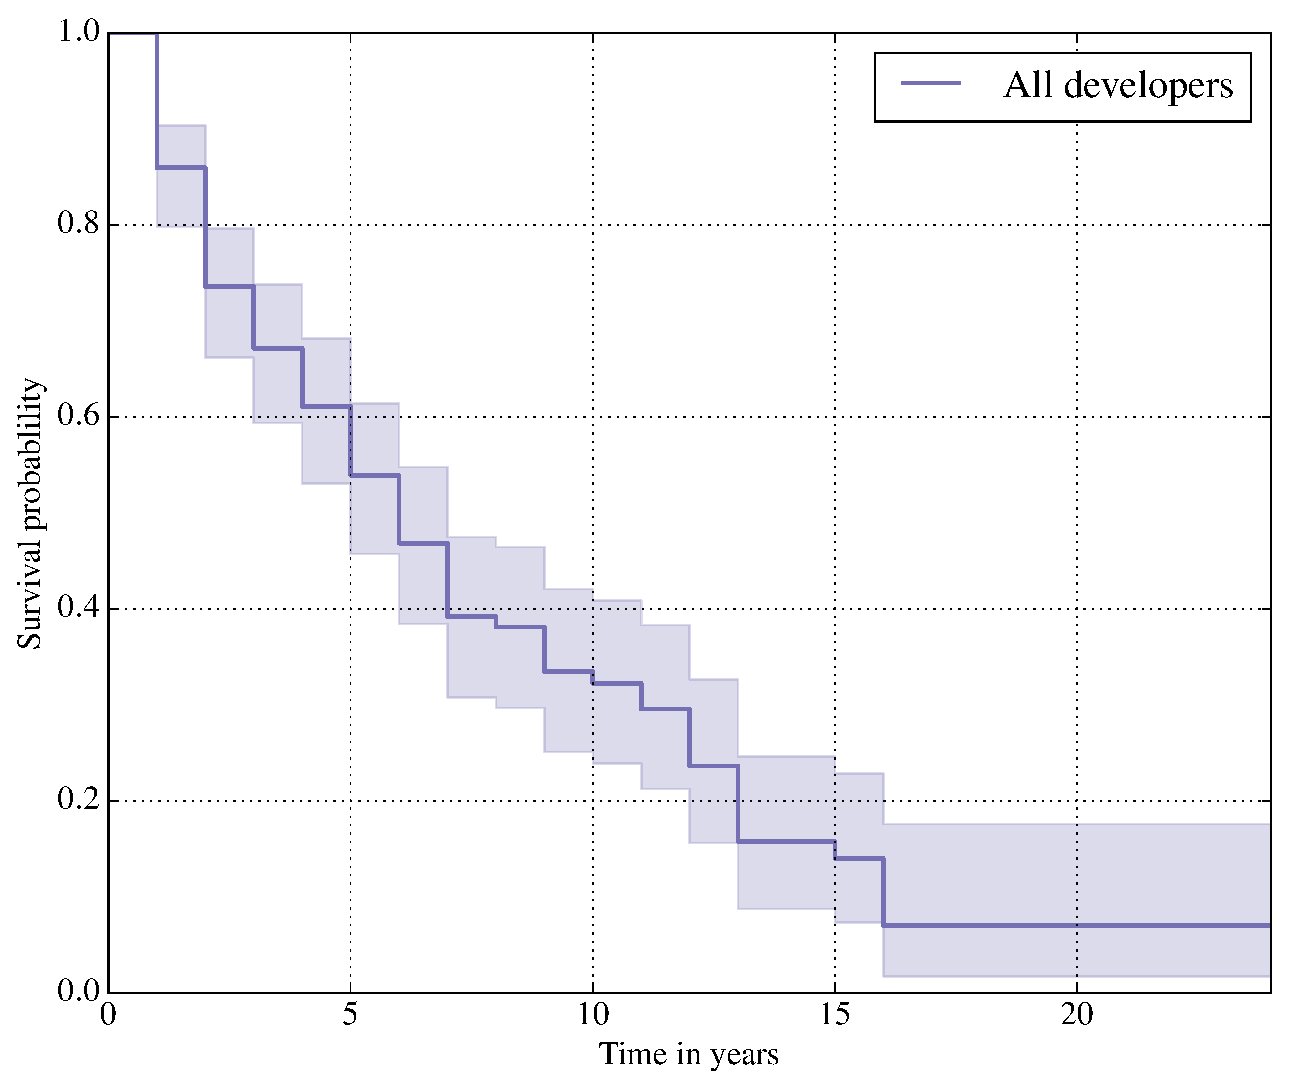
\includegraphics[scale=0.2]{../../figures/survival_all}
}
\hspace{.01in}
\subfloat[Survival Function for developers in the top connectivity level]{
\label{fig:survival_groups}
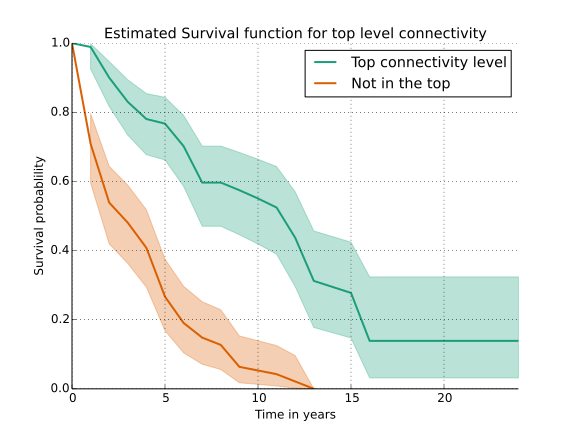
\includegraphics[scale=0.2]{../../figures/survival_top}
}
\label{fig:survival}
\caption[Survival function using the Kaplan-Meier estimate.]{Estimation of the survival function using the Kaplan-Meier estimate. The median survival time of a developer in the community, defined as the point in time where on average half of the population has abandoned the community, is 6 years if I consider all developers (left). But if I consider separately the developers in the top level of the connectivity hierarchy (right), their median survival time is 12 years; but only 3 years for the developers that are not on the top of the connectivity hierarchy.}
\end{figure}



\end{frame}

%\section{References}

\begin{frame}[label=biblio]
\frametitle{References}
% Bibliografia
\begin{footnotesize}
\bibliographystyle{chicago}
\bibliography{../../thesis.bib}
\end{footnotesize}
\end{frame}

\end{document}
